%----------------------------------------------------------------------------------------
%	PACKAGES AND THEMES
%----------------------------------------------------------------------------------------
\documentclass{beamer}
\usetheme{Boadilla}

\usepackage{hyperref}
\usepackage{graphicx}
\usepackage{booktabs}
\usepackage{amsmath}
\usepackage{tikz}
\usepackage{pgfplots}
\pgfplotsset{width=7.5cm,compat=1.12}

%----------------------------------------------------------------------------------------
%	TITLE PAGE
%----------------------------------------------------------------------------------------

% The title
\title{Research Presentation}
\subtitle{Using Beamer}

\author{Alejandro Gonzalez and Shoaib Laghari}
\institute{University of Washington and Washington University}
\date{\today} % Date, can be changed to a custom date

%----------------------------------------------------------------------------------------
%	PRESENTATION SLIDES
%----------------------------------------------------------------------------------------

\begin{document}

\begin{frame}
    % Print the title page as the first slide
    \titlepage
\end{frame}

\begin{frame}{Agenda}
    \tableofcontents
\end{frame}

\section{Learning by doing}
\subsection{Previous literature}
\begin{frame}{Learning by doing: Overview}
    Task: find estimates of $\eta$ in Alejandro's simplified model
    \[ Y_t = A_t (1- u_t) \hspace{3cm} (1) \] 
    \[ A_t = exp(\phi) A_{t-1} (1 - u_{t-1})^{\eta} \hspace{1cm} (2) \]
    \newline
    \newline
    $\eta$: measure of the impact that previous GDP/employment (in time t-1) has on current technology (time t)
\end{frame}

\begin{frame}{Learning by doing: Previous literature}
    \begin{itemize}
        \item Journals
        \begin{itemize}
            \item Econometrica
            \item American Economic Review
            \item Journal of Political Economy
            \item Journal of Monetary Economics
        \end{itemize}
        \item Timeline of LDB Literature
        \begin{itemize}
            \item 30s-40s: Wright and Middleton, aircraft industry; Searle, shipbuilding
            \item 50s: Development of Wright's model
            \item 60s-80s: Empirical Studies of LBD in various industries
            \item 90s: Spillover effects
            \item 2000s-2010s: Organizational forgetting
        \end{itemize}
    \end{itemize}
\end{frame}

\begin{frame}{Learning by doing: Previous literature}
    \begin{itemize}
        \item Where's the data being collected?
        \begin{itemize}
            \item Shipyards
            \item Assembly plants (automobiles, semic-conductors)
            \item Aircraft production facilities
            \item Energy technology
        \end{itemize}
        \item Sample Specifications
        \begin{itemize}
            \item Production functions and progress ratios
        \end{itemize}
    \end{itemize}
    \vspace{0.5cm}
    T.P. Wright (JAS, 1936)
    \[ Y = aX^b \hspace{1.5cm} (3) \]
    \[ p = 1 - 2^{-\beta} \hspace{1cm} (4) \]
\end{frame}
% Typically, production costs are reduced sometimes by orders of magnitude. This phenomenon was first described by Wright: he reported that unit labour costs in airframe manufacturing declined significantly with accumulated experience of the workers, and also that this cost reduction was a constant percentage with every doubling of cumulative output.

% From these curves one deduces the so-called ‘progress ratio’ (p), which is the relative amount of cost reduction per doubling of cumulative output.

\begin{frame}{Learning by doing: Previous literature}
    \begin{itemize}
        \item Where's the data being collected?
        \begin{itemize}
            \item Shipyards
            \item Assembly plants (automobiles, semic-conductors)
            \item Aircraft production facilities
            \item Energy technology
        \end{itemize}
        \item Sample Specifications
        \begin{itemize}
            \item Production functions and progress ratios
        \end{itemize}
    \end{itemize}
    \vspace{0.5cm}
    Rapping (AER, 1965)
    \[ ln{X_{it}} = ln{A} + \lambda t_1 ln{e} + \beta_1 ln{M_{it}} (5) + \beta_2 ln{K_{it}} + \beta_3 \sum_{t=0}^{T-1} X_t + ln{V_{it}} \hspace{0.5cm} (5)\]
\end{frame}

\begin{frame}{Learning by doing: Previous literature}
    \begin{itemize}
        \item Where's the data being collected?
        \begin{itemize}
            \item Shipyards
            \item Assembly plants (automobiles, semic-conductors)
            \item Aircraft production facilities
            \item Energy technology
        \end{itemize}
        \item Sample Specifications
        \begin{itemize}
            \item Production functions and progress ratios
        \end{itemize}
    \end{itemize}
    \vspace{0.5cm}
    Cooper and Johri (JME, 2002)
    \[ \Delta TFP_{it} = \gamma \Delta TFP_{it-1} + \varepsilon \eta \Delta y_{it-1} + \Delta a_{it} \hspace{1cm} (6)\]
\end{frame}

\begin{frame}{Learning by doing: Estimates}
    \begin{columns}[c]
        \column{.5\textwidth} % Left column and width
            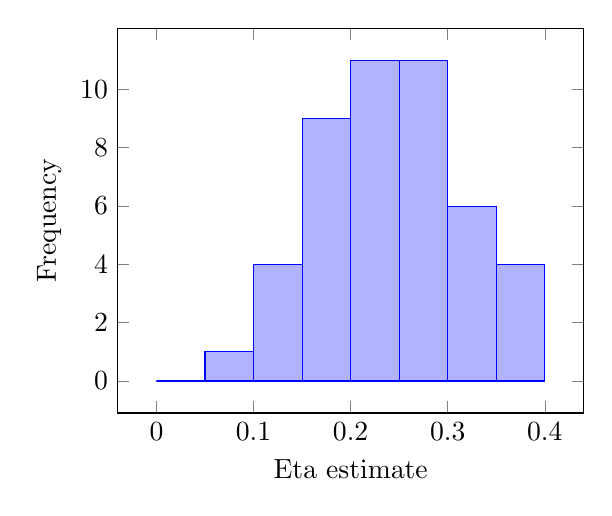
\begin{tikzpicture}
                \begin{axis}[
                    area style,
                    xlabel = Eta estimate,
                    ylabel = Frequency,
                    ytick={0, 2, 4, 6, 8, 10}
                    ]
                \addplot+[ybar interval, mark=no] coordinates { 
                    (0, 0)
                    (.05, 1)
                    (.10, 4)
                    (.15, 9)
                    (.2, 11)
                    (.25, 11)
                    (.3, 6)
                    (.35, 4)
                    (.4, 4)
                };
                \end{axis}
            \end{tikzpicture}
        \column{.3\textwidth} % Right column and width
            \begin{itemize}
                \item Mean: .235
                \item Median: .233
                \item Older data
            \end{itemize}
    \end{columns}
\end{frame}

\subsection{Limitations}

\begin{frame}{Learning by doing: Limitations}
    A limitation of the estimates collected is that they rely on manufacturing data, which is only $1/3$ of US production.
    \newline
    \newline
    Could be okay, though, because Kaldor (1978) also relies on manufacturing sector to explain productivity growth.
    \newline
    \newline
    Is translating estimates from previous literature into the aggregate economy reasonable?
\end{frame}
% From Kaldor (1978): 
% "Increasing returns is by far the more important cause of differences in productivity growth rates; differences in investment behavior explain residual differences which are relatively less important."
% "I am not suggesting that the Verdoorn relationship applies only to manufacturing activities... but its application outside the industrial field is clearly far more limited."
% "There remains the tertiary sector, services, comprising such divergent items as transport, distribution, banking and insurance, catering and hotels, laundries and hairdressers, and professional services of the most varied kind..."

\section{Issues to consider}
\subsection{Organizational forgetting}
\subsection{Learning spillovers}

\begin{frame}{Issues to consider: Forgetting and Spillovers}
    C.L. Benkard (AER, 2000) - Learning and Forgetting: The Dynamics of Aircraft Production
    \[ ln{L_i} = ln{A(\overline{K})} + \theta ln{E_i} + \gamma_0 ln{S_i} + \varepsilon_i \hspace{1cm} (7)\]
    , and 
    \[ E_i = 
    \begin{Bmatrix} 
        \hspace{0.7cm} E_{1, t} :$ if i is type $-1, -100, -200\\
        \hspace{0.7cm} E_{500, t} :$ if i is type $-500 \hspace{2cm}
    \end{Bmatrix} 
    \]
    , where
    \[ E_{1,t} = \delta E_{1,t-1} + q_{1,t-1} + \lambda q_{500,t-1} \hspace{1cm} (8) \]
    \[ E_{500,t} = \delta E_{500,t-1} + q_{500,t-1} + \lambda q_{1,t-1} \hspace{1cm} (9) \vspace{0.5cm}\]
    $\delta$ = 1.0 and $\lambda$ = 1.0 correspond to no organizational forgetting and complete spillovers, respectively. 
\end{frame}

\begin{frame}{Issues to consider: Organizational Forgetting}
Eta here is a combination of multiple coefficients (their learning, forgetting, AND spillovers).
\newline
\newline
Estimated learning coefficient (0.36) is misleading because our definition assumes no forgetting/spillovers.
\newline
\newline
Other specifications: Cooper and Johri (2002), Levitt (2013), Irwin and Klenow (1994), Thornton and Thompson (2001) 
\end{frame}

\begin{frame}{Issues to consider: Coefficient Estimates}
    \begin{table}
        \begin{tabular}{l l l}
            \toprule
            \textbf{Author (year)} & \textbf{Forgetting} & \textbf{Spillovers} \\
            \midrule
            Cooper (2002)         & 0.985          & 0.562               \\
            Levitt (2013)         & 0.965           & 0.41               \\
            Irwin (1994)         & 0.98           & 0.29             \\
            Benkard (1994)         & 0.92          & 0.32              \\
            \bottomrule
        \end{tabular}
        \caption{Estimates of forgetting and spillovers}
    \end{table}
\end{frame}

\section{Extending FFV CJE}
\begin{frame}{Extending FFV CJE}
Key items:
\newline
\newline
How to extend Steve's model to account for spillovers and forgetting
\newline
\newline
Adjusting our learning estimate (.25) to account for forgetting
\end{frame}

%----------------------------------------------------------------------------------------

\end{document}

